%%%%%%%%%%%%%%%%%%%%%%%%%%%%
%% Event generation 
%%%%%%%%%%%%%%%%%%%%%%%%%%%%


In this section I will explain in more detail the various techniques employed by the most common
event generators. In particular, I will focus on \MADGRAPH~\cite{Alwall:2011uj,Alwall:2014hca} and
\PYTHIA~\cite{Sjostrand:2006za}, the programs that generated the events for most of the processes
used in the Razor Boost analysis, presented in Chapter~\ref{chap:razorboost}. 
The following sections are based on
Refs.~\cite{Campbell:2006wx,Salam:2010zt,Skands:2011pf,Buckley:2011ms,Sjostrand:2006za,Alwall:2011uj
,Alwall:2014hca}. 

\subsection{Matrix element generators \label{sec:event_matrix_element_generators}}

As explained previously, the hard interaction can be described using matrix elements, which can be
computed, at least in principle, order by order using perturbation theory. 
There are a variety of programs available that calculate the tree-level diagrams numerically,
and integrate over the relevant phase space. The most widely used are \MADGRAPH, now merged
into \textsc{MG\_aMC@NLO}, and \textsc{Alpgen}~\cite{Mangano:2002ea}. 
There are no inherent limits to the number of final state particles that could be produced with
these programs, although, in practice, the computation is limited by the factorial growth of the
number of diagrams as we go higher in multiplicity of final state particles. 
In this section I will explain the basic algorithms used by \MADGRAPH to generate events at leading
order accuracy. For all details, and a discussion on how event generation at next-to-leading order
precision is done, I refer to Refs.~\cite{Alwall:2011uj,Alwall:2014hca}.

\MADGRAPH allows for automatic generation of matrix elements for collider physics processes, such as
decays and $2 \rightarrow n$ scatterings. 
As the user, one first specifies the desired process in terms of initial and
final state particles. It is possible to exclude or require the presence of s-channel resonances,
and one can force a particular decay chain. 
Once the process is fully specified, \MADGRAPH computes all Feynman diagrams that can contribute,
and writes process-specific code to compute the matrix elements. The user is not restricted
to models implemented by default in \MADGRAPH. Feynman rules for any (new) physics model can be
obtained via \textsc{FeynRules}~\cite{Alloul:2013bka} and passed to \MADGRAPH via the standardized
UFO format~\cite{Degrande:2011ua}. 

The algorithm to determine all relevant diagrams recursively creates sub-diagrams by merging legs.
It can be most easily explained by considering a simple example. We will go through the different
steps for the diagram generation of $e^+ e^- \rightarrow \cPqu \cPaqu \cPg$. The relevant vertices
in the Standard Model are $(e^+ e^- \gamma)$, $(e^+ e^- \cPZ)$, $(\cPqu \cPaqu \gamma)$, $(\cPqu
\cPaqu \cPZ)$, and $(\cPqu \cPaqu \cPg)$. Before the start of the algorithm, the initial state
particles are flipped such that only outgoing particles are present. We then proceed as follows.
\begin{enumerate}
  \item  First it is checked whether there is a vertex including all particles. In this example
this is not the case. 
  \item Then all possible two-particle groupings are performed, and the groups are replaced by a
single particle according to the allowed vertices. An example is the grouping $(e^+ e^-) \cPqu
\cPaqu \cPg$, which results in the replacements $(\gamma) \cPqu \cPaqu \cPg$ and $(\cPZ) \cPqu
\cPaqu \cPg$. The full list of groupings and replacements for this example is shown in
Table~\ref{tab:madgraph_diagrams}. Each option gets assigned a number according to how many groups
were replaced, here either 1 or 2. 
  \item All combinations after the replacement for which fewer than two groupings were replaced,
i.e. the first seven in the table, are discarded because they cannot give rise to valid diagrams, or
would lead to double counting if grouped further. 
  \item For the remaining combinations the presence of a valid vertex is checked. Only the final
four options have a valid vertex in this example. These diagrams are thus added to the list of
possible diagrams. 
  \item The iteration ends here because any further grouping of these valid diagrams would result
in a state that contained less than two replacements. The four diagrams that were generated are
shown in Fig.~\ref{fig:madgraph_diagrams}.
\end{enumerate}

\begin{table}[t]
  \caption{Steps for the diagram generation algorithm employed in \MADGRAPH. Table taken from
Ref.~\cite{Alwall:2011uj}. 
  \label{tab:madgraph_diagrams}}
  \begin{center}
  {\setlength{\tabcolsep}{1.5eM}
  \begin{tabular}{l l l}
  \toprule
  First iteration & Groupings & Replacements \\
  \midrule
  \multirow{17}{*}{$e^-,e^+,\cPqu,\cPaqu,\cPg$} & \multirow{2}{*}{$(e^-,e^+),\cPqu,\cPaqu,\cPg$} &
$(\gamma), \cPqu, \cPaqu, \cPg$ \\
  & & $(\cPZ), \cPqu, \cPaqu, \cPg$ \\ \cmidrule(lr){2-3}
  & \multirow{3}{*}{$e^- , e^+ , (\cPqu, \cPaqu), \cPg$} & $e^- , e^+ , (\gamma), \cPg$ \\
  & & $e^- , e^+ , (\cPZ), \cPg$ \\
  & & $e^- , e^+ , (\cPg), \cPg$\\ \cmidrule(lr){2-3}
  & $e^- , e^+ , (\cPqu, \cPg), \cPaqu$ & $e^- , e^+ , (\cPqu), \cPaqu$\\ \cmidrule(lr){2-3}
  & $e^- , e^+ , \cPqu, (\cPaqu,\cPg)$ & $e^- , e^+ , \cPqu, (\cPaqu)$\\ \cmidrule(lr){2-3}
  & \multirow{6}{*}{$(e^- , e^+ ), (\cPqu, \cPaqu), \cPg$} & $(\gamma), (\gamma), \cPg$ \\
  & & $(\gamma), (\cPZ), \cPg$\\
  & & $(\gamma ), (\cPg), \cPg$\\
  & & $(\cPZ ), (\gamma), \cPg$\\
  & & $(\cPZ ), (\cPZ), \cPg$\\
  & & $(\cPZ ), (\cPg), \cPg$\\ \cmidrule(lr){2-3}
  & \multirow{2}{*}{$(e^- , e^+ ), (\cPqu, \cPg), \cPaqu$} & $(\gamma ), (\cPqu), \cPaqu$\\
  & & $(\cPZ ), (\cPqu), \cPaqu$ \\ \cmidrule(lr){2-3}
  & \multirow{2}{*}{$(e^- , e^+ ), \cPqu, (\cPg, \cPaqu)$} & $(\gamma ), \cPqu, (\cPaqu)$\\
  & & $(\cPZ ), \cPqu, (\cPaqu)$\\ 
  \bottomrule
  \end{tabular}
  }
  \end{center}
\end{table}

\begin{figure}
  \centering
  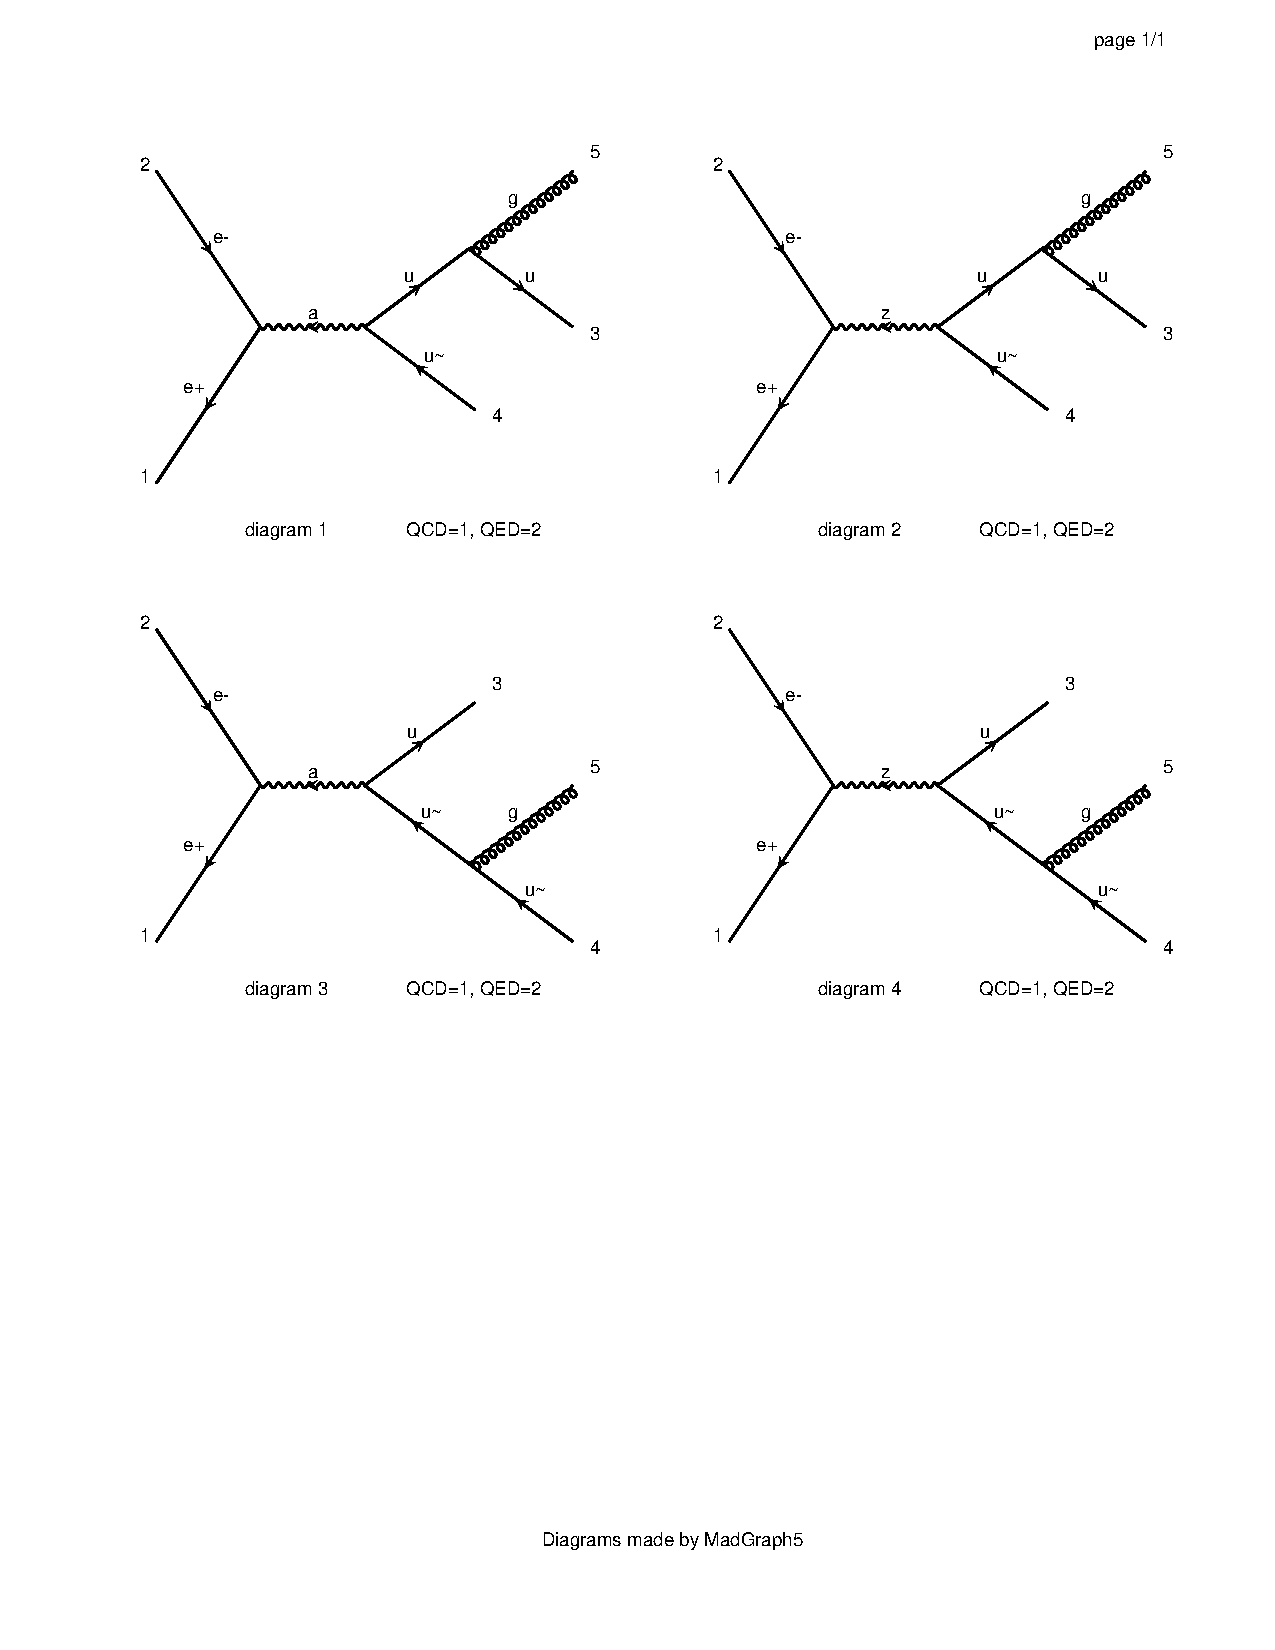
\includegraphics[width=0.9\textwidth, clip=true, trim=1cm 10.5cm 1cm 2cm]
{figures/eventreco_generation/matrix1}
  \caption{Feynman diagrams for the process $e^+ e^- \rightarrow \cPqu \cPaqu \cPg$
  \label{fig:madgraph_diagrams}}
\end{figure}

The computation of the squared matrix element for a given process is done via calls to helicity
wavefunctions and amplitudes. Helicity amplitudes work on the amplitude level, in contrast to the
methods using contraction of Lorentz-indices that work on squared amplitudes.  A big advantage is
that the complexity of the calculation grows linearly rather than quadratically, and that diagrams
are factorized such that the subcomponents, i.e. the helicity wavefunction calls, can be reused
between diagrams. 
A helicity wavefunction is first generated for each external leg in any diagram using the
\textsc{ALOHA}~\cite{deAquino:2011ub} package. 
These wavefunctions are then combined into new wavefunctions corresponding to the propagators in the
diagram by successive helicity wavefunction calls. The final vertex then corresponds to a helicity
amplitude call which returns the value of the amplitude corresponding to this particular diagram.

Particle decays are treated in the same way as the production, allowing for efficient treatment of
multiprocesses with the same decay pattern. An example of this is the process $\Pp \Pp \rightarrow
\W^+$, with $\W^+ \rightarrow \ell^+ \nu_l$. This process contains the production
processes, $\cPqu \cPaqd \rightarrow \W^+$, $\cPaqd \cPqu \rightarrow \W^+$, $\cPqc \cPaqs
\rightarrow \W^+$, $\cPaqs \cPqc \rightarrow \W^+$, and the decay processes $\W^+ \rightarrow
e^+ \nu_e$, $\W^+ \rightarrow \mu^+ \nu_\mu$, $\W^+ \rightarrow \tau^+ \nu_\tau$. 
All these building blocks only need to be generated once, and can then be combined in all possible
ways to obtain the full matrix element.  
 
Once the code for the process under consideration is generated, we can start generating events.
\MADGRAPH uses a so-called run\_card as configuration for the event generation. In this card the
user can specify how many events to produce, which phase space cuts to apply, which parton
distribution functions to use, how to choose the renormalization scale, etcetera. Using this
configuration, the numerical integration of the matrix element squared over the appropriate phase
space is performed, and unweighted events are finally obtained. 

The phase space to integrate is usually high-dimensional, and contains many peaks, which are often
 related to propagators in one of the diagrams becoming large. 
Efficient sampling techniques are thus critical for the performance of the event generation.
Standard MC integration techniques such as importance sampling have the drawback that you need to
know a lot about the function $f$ you wish to integrate in order to find an appropriate, more
well-behaved, function $g$ to help the MC integration. 
Since this is not usually the case for these phase space integrals, the \MADGRAPH program implements
a custom integration method, called single-diagram-enhanced multi-channel
integration~\cite{Maltoni:2002qb}.
The method works as follows.
Assume that the function to be integrated could be written in terms of a basis of $n$ functions
$f_i$,
\begin{equation}
  f = \sum_{i=1}^n f_i, \text{ with } f_i > 0, \quad \forall i,
\end{equation}
such that the peak structure of each $f_i$ can be efficiently mapped by a single function $g_i$.
Then, the integration of $f$ reduces to a sum of $n$ independent, and simpler, integrations.
\begin{equation}
  I = \int d\Phi f(\Phi) = \sum_{i=1}^n \int d\Phi g_i(\Phi) \frac{f_i(\Phi)}{g_i(\Phi)} =
\sum_{i=1}^n I_i .
\end{equation}
For a generic integration problem, such a basis might be too difficult to identify, but here we can
use the physical content of the process and decompose $f$ according to the single Feynman diagrams, 
\begin{equation}
  f_i = \frac{|A_i|^2}{\sum_i |A_i|^2} |A_{\text{total}}|^2
\end{equation}
where $A_i$ is the amplitude corresponding to a single Feynman diagram and $A_{\text{total}}$ is the
total amplitude. Finding the suitable mapping $g_i$ is straightforward, since it can be
derived from the known propagator structure of the corresponding Feynman diagram. 
Since the $I_i$ can be computed independently and then combined, this method is inherently parallel
in nature, allowing the use of computer clusters to speed up the computation and thus facilitating
the generation of more complicated processes.  

Because of its good performance, ease of use, and flexibility, \MADGRAPH is the standard
matrix-element generator used by the CMS experiment. 
Other generators are still used for dedicated processes, or to derive systematic
uncertainties on the prediction coming from the details and approximations made by the various 
event generators. 

The result of the event generation is a set of final state, hard particles. Very
soft or collinear particles cannot be computed by matrix-element generators, as the matrix element
diverges. The next section will cover parton shower programs, whose purpose is exactly to deal with
soft and collinear radiation. Section~\ref{sec:event_matching} will discuss a technique on how to
match the matrix element computation with the parton shower to obtain the best of both worlds. 



\subsection{Parton shower}

The fixed-order matrix-element MC programs discussed in the previous section provide a powerful
combination of accuracy and flexibility as long as you want to calculate infrared and collinear safe
observables -- such as jets, $\W$ or $\cPZ$ bosons, but not pions, kaons, etcetera -- and
don’t need to study regions of phase space that involve disparate physical scales. An example of
the latter could be requiring a heavy boson to have a \pt much smaller than its mass, leading to
large coefficients at all orders in the perturbative expansion.
These defects are related to the presence of soft and collinear divergences in the calculations.
Real life does not diverge, however. We thus need a different approach to tackle the soft and
collinear part of the phase space. This approach is the parton shower. 

Parton shower algorithms, such as the one implemented in \PYTHIA, describe the evolution in
momentum transfer from the high scales associated with the hard process down to the low scales, of
order 1\GeV, associated with the confinement of the partons it describes into hadrons. 
In analogy with bremsstrahlung of photons in QED, a parton (quark or gluon) with high momentum will
have some probability to radiate a gluon. This gluon can then radiate more gluons, or it can split
in a $q\bar{q}$ pair. This process repeats itself until the energy of the quarks and gluons becomes
too low, and hadronization begins. Hadronization is a non-perturbative process, but fortunately it
is universal, i.e. it does not depend on the hard interaction, but only on the partons at the low
scale after the parton shower.

The probabilities for the various parton splittings are encompassed in the splitting functions,
$P_{j\leftarrow i}$, which were already mentioned briefly in Section~\ref{sec:event_pdfs}.
Let us first introduce the variable $t$ as
\begin{equation}
  t = \ln\frac{Q^2}{\Lambda^2},
\end{equation}
with $\Lambda$ the QCD scale. We then find for the differential
\begin{equation}
  \text{d}t = \text{d}\ln Q^2 = \frac{\text{d}Q^2}{Q^2}.
\end{equation}
We can view $t$ as a kind of time in the evolution of the parton shower. The smaller $t$, and
thus the lower the scale, the further along in the shower process we are. 
In terms of the variable $t$, we can write the differential probability for a parton $i$ to branch
into any parton $j$ with momentum fraction $z$ in the following way,
\begin{equation}
  \text{d}\mathcal{P}_i = \sum_j \frac{\alpha_S}{2\pi} P_{j\leftarrow i}(z)\text{d}t\text{d}z,
\label{eq:splitting}
\end{equation}
with the different splitting functions in the collinear limit given by
\begin{align}
  P_{q\leftarrow q}(z) &= C_F \frac{1 + z^2}{1 - z}, & 
  P_{g\leftarrow q}(z) &= C_F \frac{1 + (1-z)^2}{z}, \\
  P_{g\leftarrow g}(z) &= C_A \frac{z^4 + 1 + (1-z)^4}{z(1-z)}, &
  P_{q\leftarrow g}(z) &= T_R (z^2 + (1-z)^2), 
\end{align}
where $C_F$ and $C_A$ are colour factors and $T_R$ is a constant depending on the definition of
$\alpha_S$. 
There are two sets of divergencies that occur in the computation of the branching probability: when
the radiated parton becomes extremely soft, or when it becomes collinear with the original parton. 
The cases where this occurs can in fact not be resolved in any physical measurement. Two exactly
collinear partons look exactly like one parton with the same total momentum. We should thus impose
a resolution criterion. Often the chosen criterion is that the relative transverse momentum
between the two partons is larger than some cutoff scale $Q_0$. Imposing this cutoff, then results
in a finite resolvable emission probability. Because the total probability of something happening
has to be unity, we can find the probability to not have a resolvable emission as one minus the
resolvable emission probability. In this way we have avoided computing the divergent pieces, which
would have to be added to the divergent loop-correction to the hard process in order to cancel.

Since Eq.~\ref{eq:splitting} is a completely general expression that does not depend on the hard
process, we can iterate it, using it on a parton resulting from the hard process to generate
one branching and then treating the new final state as the hard process, generating another
splitting from it, and so on. In what follows we will discuss how this shall be done in practice.

The integral of the branching probability over all allowed $z$ values, according to the
particular resolution criterion imposed, and for a given $t$ value, is defined as
\begin{equation}
  \mathcal{I}_{j\leftarrow i}(t) = \int dz \frac{\alpha_S}{2\pi} P_{j\leftarrow i}(z)
\end{equation}
The naive probability that a resolved branching occurs during a small range of $t$ values, $\delta
t$, is given by 
\begin{equation}
 \sum_j \mathcal{I}_{j\leftarrow i}(t) \delta t,
\end{equation}
where we did not take into account anything which could have happened during the parton shower,
before that time. The probability for no resolved emission to occur is then simply given by $1 -
\sum_j \mathcal{I}_{j\leftarrow i}(t) \delta t$. 
If the evolution of parton $i$ starts at $t_{\text{max}}$, then the probability that the parton
has not yet branched later in the shower, when $t < t_{\text{max}}$, is given by
the product of the probabilities that it did not branch in any of the small intervals $\delta t$
between $t$ and $t_{\text{max}}$. In other words, letting $\delta t \rightarrow 0$, the no-branching
probability at time $t$, given starting point $t_{\text{max}}$, exponentiates, and is given by
\begin{equation}
  \mathcal{P}_{\text{no-branching}}(t_{\text{max}},t) = \exp 
  \left\{ - \int_t^{t_{\text{max}}} dt' \sum_j \mathcal{I}_{j\leftarrow i}(t') \right\} .
\end{equation}
The actual differential probability that the first resolved branching of parton $i$ occurs at `time'
$t$, which is the actual question we wish to answer, is thus given by
\begin{align}
  \frac{\text{d}\mathcal{P}_i}{\text{d}t} &= -
\frac{\mathcal{P}_{\text{no-branching}}(t_{\text{max}},t)}{\text{d}t} \\
 &= \left( \sum_j \mathcal{I}_{j\leftarrow i}(t)\right) \exp \left\{ - \int_t^{t_{\text{max}}} dt'
\sum_j \mathcal{I}_{j\leftarrow i}(t) \right\}, \label{eq:prob_first_branch}
\end{align}
where the first factor in Eq.~\ref{eq:prob_first_branch} is the naive probability mentioned above,
and the second term is an exponential suppression, similar to that found in the formula for
radioactive decay, to account for the fact that if a parton has already branched at $t'$, it can no
longer branch at $t$. 
This exponential factor, the probability to not branch above a certain scale, here
contained in the variable $t$, is called the Sudakov form factor, $\Delta_i(t_max,t)$. 

Implementing this in a Monte Carlo program is conceptually straightforward. 
First, a random number $r$ is sampled uniformly between 0 and 1. Then the value for $t$ such that 
$\Delta_i(t_max,t) = r$ is determined. If the solution is above the cutoff $t_0$, corresponding to
the resolution $Q_0$, then a resolvable branching is generated with scale $t$, otherwise the shower
evolution is terminated. In case a resolvable branching is to be generated, a $z$ value is chosen
according to the splitting functions $P_{j\leftarrow i}(z)$, and then the algorithm is started
again. 
Of course, in practice one has to take into account several complications. 
Different approaches exist for deciding what the initial scale $t_{\text{max}}$ should be.
This scale has to match the hard interaction, and could thus be the largest virtuality in the hard
scatter, but could also be the centre-of-mass energy. 
The Sudakov form factor is also not necessarily easily invertible analytically, which can dealt
with by using the so-called veto-algorithm. 
Apart from final state
showers, such as explained here, the initial state also undergoes showering. There it is important
to properly match the parton shower with the PDF treatment, as well as ensure on-shell partons that
take part in the hard interaction.
For all details on how this is fully implemented in the \PYTHIA shower routine, I refer to
the manual~\cite{Sjostrand:2006za}. 

At the end of the parton shower procedure, we end up with many more partons than we had directly
after the hard interaction, all which should be described at the low scale, via non-perturbative
models. The most widely used hadronization model will be discussed in
Section~\ref{sec:event_hadronization}. 


\subsection{Matching the matrix element to the parton shower \label{sec:event_matching}}

On the one hand, parton shower MC programs provide an excellent event description in regions which
are dominated by soft and collinear gluon emission, including the hadron-level details that are
necessary for the proper simulation of detector effects. 
On the other hand, matrix element calculations provide a good description of processes where
the partons are energetic and widely separated. They also include the effects of
interference between amplitudes with the same external partons. 
The best possible event description can thus only be achieved by combining both approaches.
However, the direct addition of the two techniques can lead to double-counting in kinematic regions
where the two calculations overlap. This is of particular importance when merging samples for
different parton multiplicities, as illustrated in Fig.~\ref{fig:overlap}.
We will thus need a matching between the matrix element
and the parton shower to ensure the proper removal of these overlaps.
There are several techniques available to perform this matching. I will focus here on the so-called
\textit{MLM matching}~\cite{Alwall:2007fs}, which is the technique used in CMS to match \MADGRAPH
with \PYTHIA. The MLM technique comprises three main steps, the first of which is done at the
matrix element level. Then the partons are showered, and finally the shower jets are matched to the
hard partons. 
In next paragraphs I will discuss each step in more detail. 


\begin{figure}[t]
  \centering
  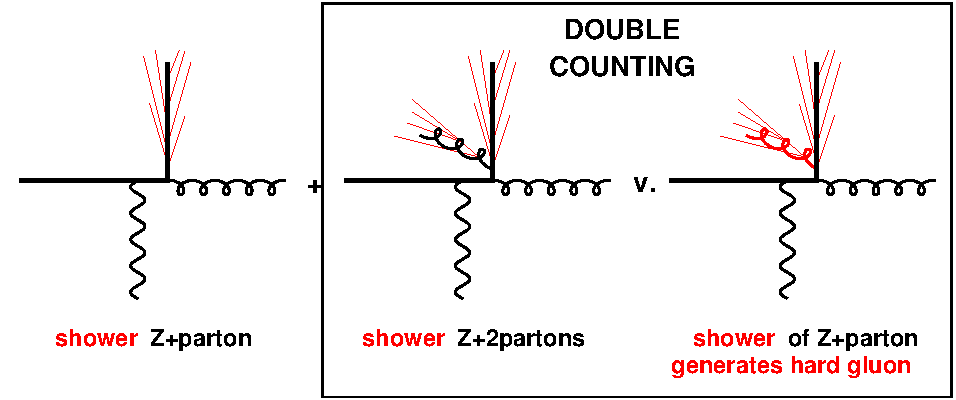
\includegraphics[width=0.8\textwidth]{figures/eventreco_generation/overlap}
  \caption{ Illustration of the double-counting issues that can arise if one naively attempts to
shower $\cPZ+$parton and $\cPZ+2$parton events. Partons generated by the matrix element are
shown in black, whereas the effects of the parton shower are shown in red. Showering the 1-parton
sample could lead to the generation of a hard gluon, which is already included in the matrix-element
description of the 2-parton sample, leading to a double-counting. Figure taken from
Ref.~\cite{Salam:2010zt}. 
  \label{fig:overlap}}
\end{figure}


For each event generated by \MADGRAPH according to the considered hard process, we want to
find out how it looks from a parton shower point of view to ensure a smooth transition from the
matrix element to the parton shower dominated region.
To arrive at this ``equivalent parton shower history", we cluster the final state partons. 
The clustering is performed using the $k_\text{T}$ jet algorithm, which defines the following two
distance measures,
\begin{align}
  k^2_{\mathrm{T},i\text{beam}} &= p_{\mathrm{T},i}^2 + m_i^2, \\ 
  k^2_{\mathrm{T},ij} &= \Delta R_{ij} \min (p_{\mathrm{T},i}^2 , p_{\mathrm{T},j}^2) + \max (m_i^2,
m_j^2),
\end{align}
with $\Delta R^2_{ij} = 2 (\cosh \Delta y - \cos \Delta\phi)$. The standard $k_\text{T}$ clustering
starts by finding the smallest of the $k^2_{\mathrm{T},ij}$ or $k^2_{\mathrm{T},i\text{beam}}$, and
combining those two partons $i$ and $j$. The combination then replaces the original two partons, and
the clustering is repeated. This continues until there is only a $2 \rightarrow 1$ or $2 \rightarrow
2$ scattering left.
A modification to the standard $k_\text{T}$ clustering is that only clusterings corresponding to
actual Feynman diagrams of the considered model are included. Two quarks of different flavour will
thus never be clustered, even if they would have the smallest $k^2_{\mathrm{T},ij}$. 
Once the clustering is performed, the smallest $k_\mathrm{T}$ value found must be larger than a
chosen cutoff scale, $Q_{\mathrm{cut}}^{\mathrm{ME}}$, otherwise the event is rejected. This cutoff
scale is called \texttt{xqcut} in the \MADGRAPH configuration files. 

In order to mimic the parton shower behaviour, the $k_\mathrm{T}$ value for each clustering vertex
associated with a QCD branching is used as new renormalization scale for $\alpha_S$ in that
vertex. This effectively results in an event reweighting. 
All factorization scales, and the renormalization scale for the hard process, i.e. without
additional partons, are constructed by clustering back to the irreducible $2 \rightarrow 2$ system,
and by using the transverse mass in the resulting frame $\mu^2 = \pt^2 + m^2$. 
At this point, the events are ready to be transferred to the parton shower. 
The clustering scales are written in the output file, such that this information is passed along to
\PYTHIA. 

% TODO figure out exact reason to use xqcut; is it for efficiency? or are there other effects as
% well

Once the events are passed to \PYTHIA, they are showered, using the factorization scale from the
previous step as starting point for the shower. Then, before hadronization starts, the showered
partons are clustered using the same $k_{\mathrm{T}}$ algorithm as before. The resulting jets are
required to have a transverse momentum larger than the \textit{matching scale} $Q_{\mathrm{match}}$,
with $Q_{\mathrm{match}} > Q_{\mathrm{cut}}^{\mathrm{ME}}$. 
Partons with a heavy quark as mother are excluded from the clustering. 

At this stage, the only missing part is the actual matching between the hard partons, and the jets
resulting from clustering the showered partons. Starting from the hardest parton $p$, we find the
closest jet $j$ and declare a match if $k_{\mathrm{T}}(j,p) < Q_{\mathrm{match}}$. We then remove
the jet, and repeat for the next hardest parton. If a parton cannot be matched to a jet, we reject
the event. 
If we can match all partons, and there are no additional jets, the event is accepted. 
In case all partons are matched, but there is an additional jet, then we need to be more careful. 
If the full process we generated had up to $N$ additional partons at the matrix element level, and
the current event had $n < N$ hard partons, then we are in exclusive mode and the event is rejected.
The reason is that the additional jet that was added by the parton shower is actually already
included at the next multiplicity. In case the current event had $N$ hard partons, we are in
inclusive mode, and we will still accept the event as long as the added jet is softer than the
softest hard parton in the event. 
In this way any double-counting is removed. These three cases are illustrated in
Figure~\ref{fig:matching}. 

\begin{figure}[htpb]
  \centering
  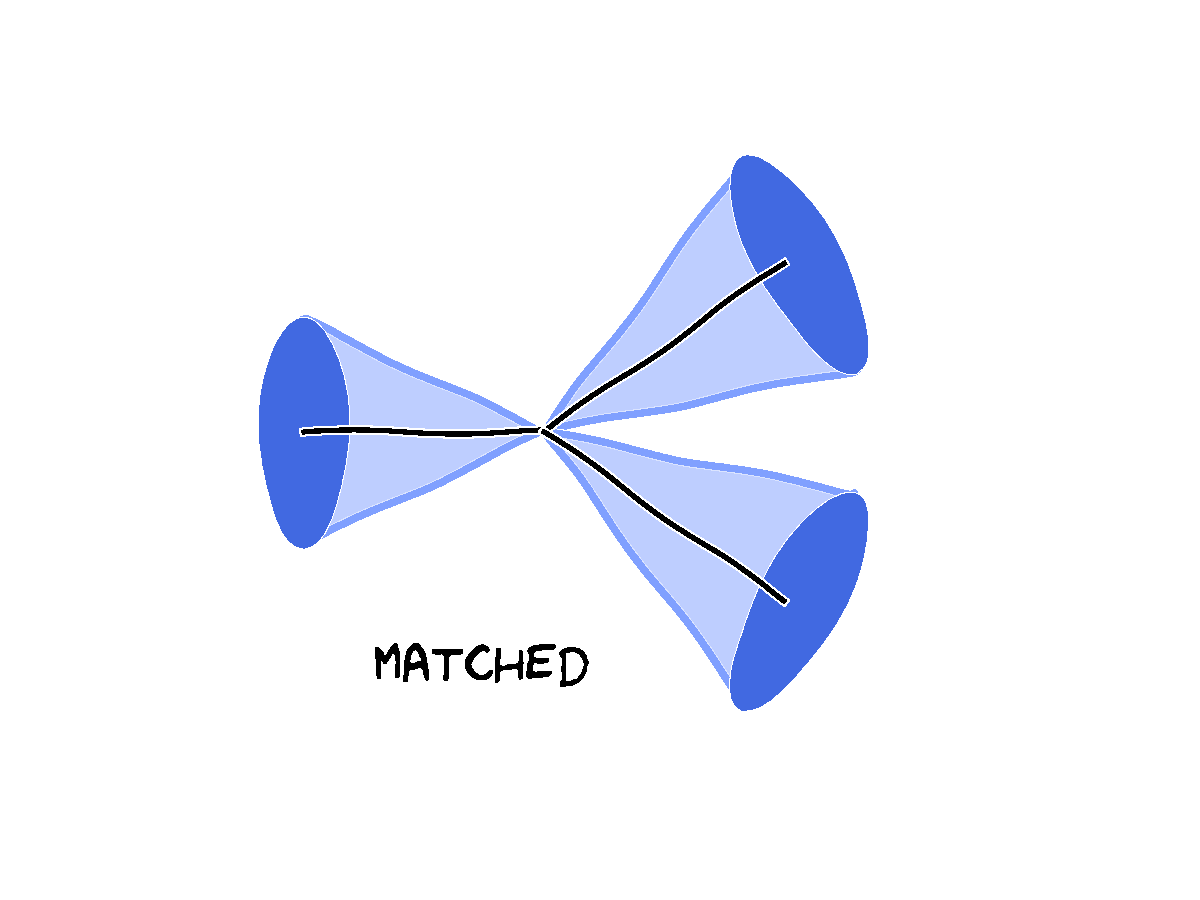
\includegraphics[width=0.31\textwidth, clip=true, trim=4cm 3cm 4cm 2cm]
  {figures/eventreco_generation/matching1}
  ~
  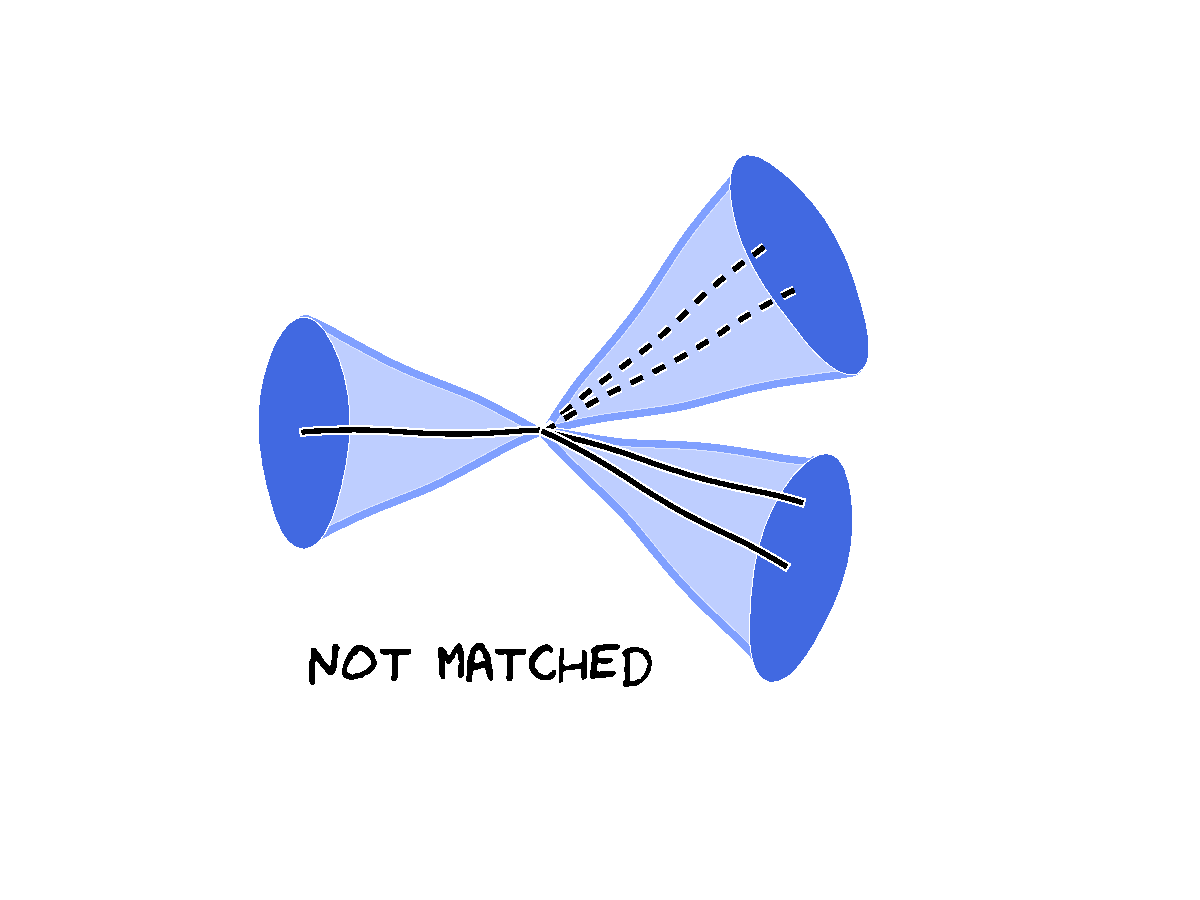
\includegraphics[width=0.31\textwidth, clip=true, trim=4cm 3cm 4cm 2cm]
  {figures/eventreco_generation/matching2}
  ~
  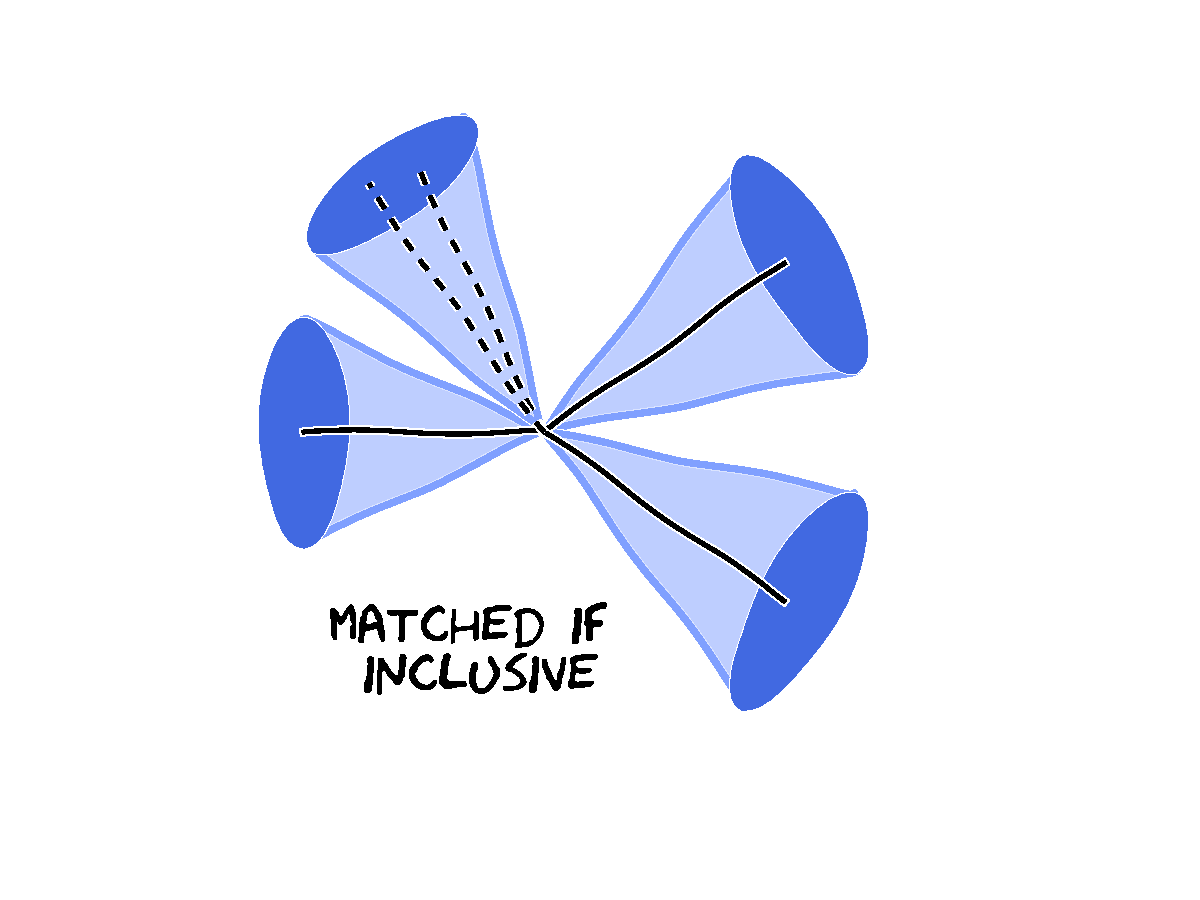
\includegraphics[width=0.31\textwidth, clip=true, trim=4cm 3cm 4cm 2cm]
  {figures/eventreco_generation/matching3}
  \caption{Illustration of the matching procedure for an event with three hard partons (solid
lines). On the left the jet clustering after the shower results in three jets, that are matched to
the three partons. The full event is thus matched, and accepted. In the middle plot the parton
shower added two extra partons (dashed lines), and the hard partons were emitted closer together.
The jet clustering still results in three jets, but now one hard parton cannot be matched to a jet.
The event will thus be rejected. In the right-hand plot each hard parton is matched to a jet, but
there is an additional jet present. If we are in inclusive mode, the event is accepted, otherwise
it is rejected.  
  Figures adapted from Ref.~\cite{mlm_plots}. 
  \label{fig:matching}}
\end{figure}


It is important to verify that the matching procedure behaves properly. In particular, jet related
quantities should have a smooth shape, without any jumps. The presence of discontinuities indicates
that the scales $Q_{\mathrm{match}}$ and $Q_{\mathrm{cut}}^{\mathrm{ME}}$ are not chosen
correctly to ensure a smooth transition between matrix element and parton shower. The distributions
that are typically checked in this regard are the so-called difference jet rates
(DJR)~\cite{Alwall:2008qv}. 

The differential jet rate $i$ is the scale at which a given configuration with $n\geq i$ hard
partons passes from being reconstructed as an $i$-jet one to being reconstructed as an $(i − 1)$-jet
one. 
In this case, with $k_\mathrm{T}$ jet clustering, the differential jet rates are simply the actual
clustering scales. The $1\rightarrow 0$ differential jet rate (DJR1) is the \pt of the last
remaining jet after clustering. The $2\rightarrow 1$ differential jet rate (DJR2) is the smallest of
the \pt of the second last remaining jet and the $k_\mathrm{T}$ between the second and the first
jet, and so on for the other DJR distributions.

Another test of the matching procedure is the stability of the matched cross section when varying
the matching scale. In general, the systematic uncertainty associated to the matching procedure can
be estimated by varying the matching scale. A common choice is to vary the scale by a factor two up
or down. 


\subsection{Hadronization \label{sec:event_hadronization}}

Real events do not consist of partons but of hadrons. Therefore, the set of post-shower partons
must be transformed into a set of primary hadrons, which can then decay further. 
Hadronization is a non-perturbative transition taking place at the hadronization scale. In the
event generation context this scale is by construction identical to the cutoff (resolution) scale of
the parton shower.
Since we have no idea how to calculate the transition between partons and hadrons from first
principles, event generators use QCD-inspired phenomenological models.
Although non-perturbative QCD is not solved, we do have some knowledge of the properties
that such a solution must have. 
An important result from lattice QCD calculations is that the potential of the colour dipole field
between a charge and an anticharge appears to grow linearly with the separation of the charges, when
the separation is greater than about a femtometer. This is known as \textit{linear confinement}, and
is used as a starting point for the string model of hadronization.
The most widely used model is the Lund model, which is implemented in \PYTHIA.

Let us consider the production of a $\cPq\bar{\cPq}$ pair. As the quarks move apart,
linear confinement implies that a potential
\begin{equation}
  V(r) = \kappa r
\end{equation}
is expected at large distances $r$.  This is exactly the potential describing a
string with tension $\kappa$. We can thus interpret this as a colour flux tube that is being
stretched
between the quark and the antiquark. From hadron mass spectroscopy the string tension is
measured to be about $1\GeV/\unit{fm}$.
As the $\cPq$ and $\bar{\cPq}$ move apart, their kinetic energy is gradually converted to potential
energy, stored in the growing string spanned between them. 
Quark-antiquark fluctuations inside the string field can become real particles by absorbing energy
from the string. The original endpoint charges are then screened from each other and the
string breaks into two separate colour-singlet pieces, $(\cPq \bar{\cPq}) \rightarrow (\cPq
\bar{\cPq}') + (\cPq' \bar{\cPq})$. This process continues until only hadrons remain.
Since the string breaks are causally disconnected, they do not have to be considered in any
specific time-ordered sequence. In the Lund model, the string breaks are generated starting
with the hadrons containing the endpoint quarks, and iterating inwards towards the centre of the
string, alternating randomly between the left- and right-hand sides, allowing a single on-shell
hadron to be split off in each step. An illustration of the colour flux tube and the breakup of the
string system is shown in Fig.~\ref{fig:hadronization_string}.

\begin{figure}[htpb]
  \centering
  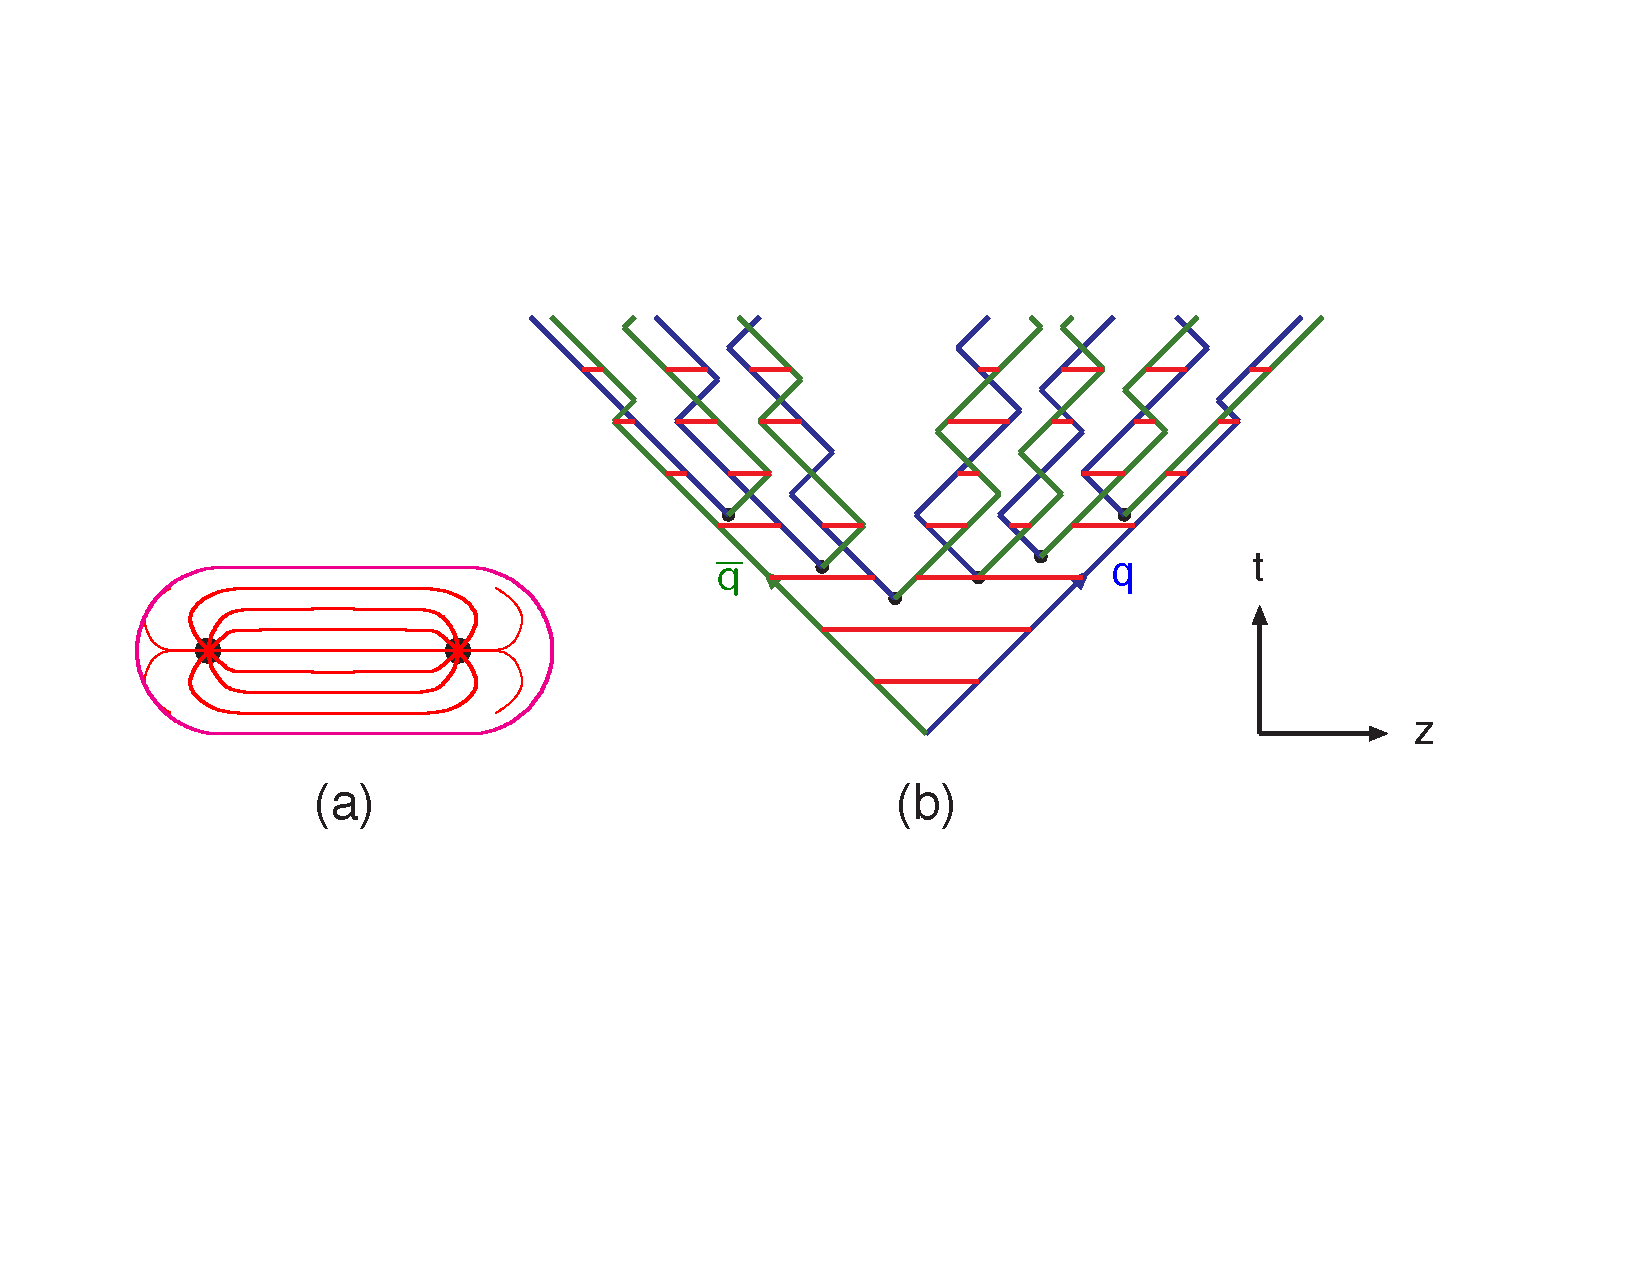
\includegraphics[width=0.8\textwidth]{figures/eventreco_generation/stringone}
  \caption{ (a) A colour flux tube spanned between a quark and an antiquark. (b) The motion
and breakup of a string system. Diagonal lines are (anti)quarks, horizontal lines snapshots of
the string field. Figure and caption taken from Ref.~\cite{Buckley:2011ms}.
  \label{fig:hadronization_string}}
\end{figure}


The details of the individual string breaks are not known from first principles. The Lund model
uses the idea of quantum mechanical tunnelling, which leads to a flavour-independent
Gaussian spectrum for the transverse momentum (w.r.t. the flux tube) of the $\cPq \bar{\cPq}$ pairs.
Baryon production can be incorporated by allowing string breaks to occur by the production of
pairs of so-called diquarks, loosely bound states of two quarks in a colour antitriplet state. 
Because the knowledge of hadronization is incomplete, experimental input is needed to tune many of
the parameters describing the finer details, such as flavour composition, and the ratio of vector to
pseudoscalar mesons. 


\subsection{Generator tuning}

Monte Carlo event generators are able to provide a full picture of collider final states, down to
the level of individual particles. This allows them to be used as theory reference against which
the Standard Model, or a new physics model, can be tested. The accuracy of the prediction depends
on the chosen observable, and on the sophistication of the generation. 
Apart from including higher order corrections, or using better non-perturbative models, it is also
crucial to constrain the remaining free parameters of the generation models using existing data.
This process is referred to as generator tuning. 

Generator models have a vast array of adjustable parameters, but most of these control relatively
small details. The few exceptions are the value of $\alpha_S$ in the perturbative domain, and the
form of the fragmentation functions that govern the non-perturbative hadronization process. 
Tuning all possible parameters is usually done in a highly factorized way, constraining just a few
parameters at a time using carefully selected experimental data. 
Of course, subsequent steps can alter the agreement obtained in the previous steps. Obtaining a
full generator tune requires several iterations. 
Automated tools have been developed in recent years to reduce the amount of manpower required.
However, the need for expert input cannot be fully removed. 

Different kinds of experimental data are used to constrain different parameters. Tuning of final
state radiation and hadronization is mostly done using LEP and other $e^+ e^-$ data,  which have
the advantage that the initial state does not cause extra complications in the interpretation of jet
related observables. Constraints on initial state radiation are derived primarily from Drell-Yan
events in hadron collisions. 
While performing the generator tuning it is important to realize that for many observables we do
not expect agreement to better than about 5-10\%. We should thus take care not to overtune on one
single observable, but rather aim for an overall adequate performance. 


